\answer{Explain briefly what is meant by the term middleware.}{2}{2013.1.a}

Software that sits in between client applications and the operating system that
abstracts the details of implementing programming tasks and masks the
heterogeneity of the underlying platforms from the client application.

\answer{Explain briefly what failures are known as Byzantine
failures.}{2}{2013.1.b}

When a remote system either:

\begin{itemize}
  \item Does not reply to messages
  \item Sends faulty replies to message with miscellaneous data
  \item Sends maliciously crafted messages
  \item Acts inconsistently when interacting with different components
\end{itemize}

\answer{Describe briefly the two-phase commit protocol.}{2}{2013.1.c}

When a client wants to commit, it sends a message to a server. The server then
asks every client whether they are ready for a commit. Each client replies with
a yes/no. If there is a no, then a \texttt{global\_abort} message is sent,
otherwise a \texttt{global\_commit} message is sent. Upon receiving a global
commit or abort message, each client does exactly that, which ensures that only
one operation is done for all clients.

\answer{What is meant when a service is provided with at least once
semantics?}{2}{2013.1.d}

The application may send the RPC call multiple times before it receives word
from the server that the RPC call has taken place and was successful. This may
result in the RPC call being executed multiple times.

\answer{Why is it practically impossible to achieve exact synchronisation of
clocks in a distributed system?}{2}{2013.1.d}

The latency in a network is variable, so you can never know exactly how long a
message took to reach a server. Because of this, if one server sends its current
clock to another server, the latter one won't know how long it took for the
message to reach it and therefore it won't know how much to increment the clock
by.

Methods such as Cristian's algorithm and the Berkeley algorithm attempt to solve
this problem, but can only do so with some assumptions and to a limited
accuracy.

\answer{When using Java RMI, what is the purpose of the RMI
registry?}{2}{2013.1.f}

To act as a central repository for computers to access remote objects. Clients
can interrogate the registry using a string and get an object back. This allows
RMI methods to have parameters that are strings that point to objects in the
repository so you can pass arbitrary data structures and objects easily.

\answer{What is meant by parameter marshalling?}{2}{2013.1.g}

When an RPC call is made, the parameters cannot be sent directly (since they may
be pointers etc), so they must be serialised into a blob of text or binary data
before they are sent (marshalled) and deserialised at the other end by the
server (unmarshalled).

\answer{What is the key difference between caching and
replication?}{2}{2013.1.h}

Replication is keeping two fully fledged entities up to date with each other in
order to provide redundancy or distribute the load of a service over more
machines.

Caching is merely a small piece of hardware or a small program that remembers
the results of expensive computations after they've been done once and returns
the result without doing any computation if the same request comes again. Rarely
is there any business logic in a cache.

\answer{Explain briefly what Little’s Law is.}{2}{2013.1.i}

Little's law dictates that the average number of elements in a queue is:

\[
  \text{av. number} = \text{av. time between arrivals} \times \text{time to process one}
\]

This allows us to estimate how a system will handle load and what its queue size
will be (and if its appropriate).

\answer{In the context of lab exercise 2, what would you do to launch a denial
of service attack against the server?}{2}{2013.1.j}

\begin{itemize}
  \item Estimate the most expensive server operation (maybe listing slots)
  \item Create a program that loops indefinitely with a request for the
    expensive operation.
  \item Run the program on a fast computer with a high bandwidth
\end{itemize}

Hopefully, the server will be too busy processing my requests to have time for
other users, therefore I would (indirectly) be denying them service.

\answer{Explain briefly why some applications are not parallelisable. Describe
Amdahl’s law and explain what it can be used for.}{4}{2013.2.a}

Amdahl's law can tell us the maximum speed up we can achieve if we parallelised
all parts of a program that don't need to be run in a serial manner.

Some parts of applications are not parallelisable because they have interactions
and data dependencies that must take place in a specific order. For example, if
we were computing the Fibonacci numbers, we couldn't parallelise it because
each new number depends on the last two, and therefore we need to know the last
two numbers before generating the next.

However, if we used the output from the Fibonacci number sequence for some
operation, say to render an image of a snail shell with Fibonacci proportions,
then the rendering could take place in parallel (since it's probably a more
intensive operation). If the Fibonacci portion of our program was about $20\%$
of computing time, and the rendering was $80\%$, then our maximum speed up would
be:

\[
  \frac{1}{0.2 + (\frac{1}{n} * 0.8)}
\]

When $n$ (the number of threads) tends to infinity (if we could use an infinite
level of parallelism), then the speed up tends towards 5.

\answer{Explain briefly what the four properties commonly denoted by the acronym
ACID are when referring to transactions.}{4}{2013.2.b}

\begin{description}
  \item \textbf{Atomicity}:\\
    A transaction either occurs (commit) or it is does not (abort), there is no
    in between. Either all of the effects of a transaction happen, or none of
    them do, which is the all or nothing principle.
  \item \textbf{Consistency}:\\
    Each transaction moves the state of the system from one valid state to
    another.
  \item \textbf{Isolation}:\\
    Even if transactions happen in parallel, they must behave as though they
    happened in a sequential manner. No transaction in progress can affect
    another transaction.
  \item \textbf{Durability}:\\
    Even in the event of a power loss, system failure or other event, once a 
    transaction is committed, it should stay committed, and not be rolled back.
\end{description}

\answer{A service is replicated onto 3 computers.
\begin{itemize}
  \item The first computer, A, has a mean time between failures of 2 days.
  \item The second computer, B, has a mean time between failures of 3.5 days.
  \item The third computer, C, has a mean time between failures of 12 days.
\end{itemize}
When a failure occurs, it takes on average 12 hours to fix.}{6}{2013.2.c}

\answer{What is the availability of the replicated service?}{2}{2013.2.c.i}

Up time of A: $\frac{48}{52}$

Up time of B: $\frac{84}{96}$

Up time of C: $\frac{288}{300}$

The down time chance is $(1 - \frac{48}{52}) * (1 - \frac{84}{96}) * (1 -
\frac{288}{300}) = \frac{1}{2600}$.

The availability is $1 - \frac{1}{2600} = 99.96\%$

\answer{What would the availability of the replicated service be if only
computers A and B were used?}{2}{2013.2.c.ii}

If only A and B were used, then the downtime would be:

\[
  d = (1 - \frac{48}{52}) * (1 - \frac{84}{96}) = \frac{1}{104}
\]

And the availability would be $1 - \frac{1}{104} = 99.04\%$

\answer{Describe how in the general case of n computers, each with a mean
time between failures if and a time to fix the failures ti you would
choose the two computers that provide the highest
availability.}{2}{2013.2.c.iii}

I would sort the computers by:

\[
  \frac{f_x}{f_x + t_x}
\]

Then I would use the top $n$ computers.

\answer{Consider the figure below, which shows 4 processes and a number of
communication events taking place over a period of time.}{6}{2013.2.d}

\begin{center}
  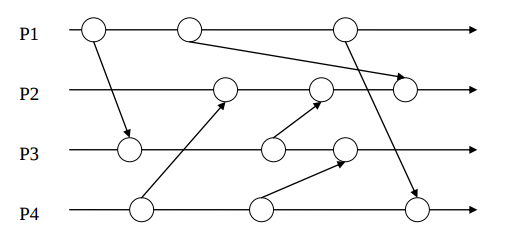
\includegraphics[width=0.5\textwidth]{images/2013-2-d}
\end{center}

\textbf{Calculate the value of Lamport clocks and vector clocks for each of the
12 events shown above. You can assume that all logical clocks start initially
with zeros.}

\begin{center}
  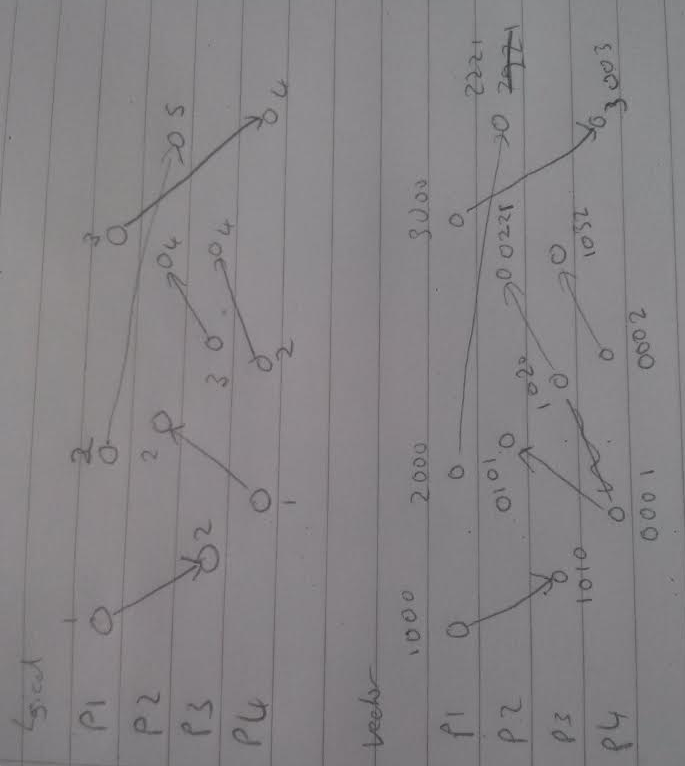
\includegraphics[angle=-90,width=0.7\textwidth]{images/2013-2-d-answer}
\end{center}

\answer{Explain briefly why the assumption “latency is zero” is considered a
common fallacy in distributed computing.}{2}{2013.3.a}

The latency between two computers can never be zero, for a number of reasons.
From a purely physical standpoint, information cannot travel faster than the
medium through which it is being carried, and even the fastest medium available
to us, light has a speed limit. Most of the time, latency is significantly
greater than the speed of light divided by the distance travelled, which is
because most of the time, the data passes through a network as packets, and is
forwarded on from node to node each time. Since multiple computers are used to
facilitate this, each one having some small amount of lag, the time between the
start point and the destination increases further. At any point along its route,
the data could get stuck in a buffer, have to take a detour etc.

Many (new) programmers haven't created applications intended to use distributed
systems before, and thus don't realise that waiting for a remote resource, RPC
call etc can (will) take orders of magnitude more time than a load from memory
might.

\answer{Describe all the operations that take place during a Remote Procedure
Call (RPC).}{5}{2013.3.b}

First, the client application will call the client stub with the procedure it
wants to execute and the parameters that are needed to do so. The client stub
then marshalls the parameters into a blob which is then sent to the server. The
server receives the message and the server stub unmarshalls the blob back into
parameters, which are then passed to the procedure on the server and the
procedure is ran. When the procedure is finished the server stub marshalls the
(possibly mutated) parameters back into a blob and sends it back to the client,
where the client stub will then unmarshal the parameters, update their values
in main memory and return to the client application.

\answer{Describe clearly how the Bully algorithm to elect a coordinator
works.}{5}{2013.3.c}

The Bully Algorithm works like this:

\begin{itemize}
\item An initiating client will send a message to all other clients with a
higher identifier than itself.
\item Any client receiving an election message will then start its own 
election, sending messages to clients with higher identifiers than itself, and 
also send an answer message back to the election message's sender.
\item Only when a process gets no replies (within a timeout) is it considered
elected. It then sends a message to all other processes announcing its election.
\end{itemize}

In this manner, any process that receives a message should always send a message
back to the sender. The upper bound on the number of messages is $O(n^2)$, and
timeouts can also make the election slow.

\answer{The following four processes access a shared variable x. Each process
accesses a different replica of the store used to hold this variable. Before any
process starts executing, the value of x is 0 in all the replicas.}{8}{2013.3.d}

\begin{center}
  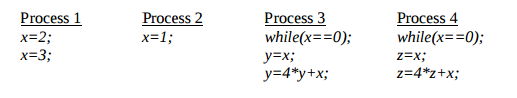
\includegraphics[width=0.5\textwidth]{images/2013-3-d}
\end{center}

\answer{When all four processes have completed executing the statements
given, are 6 and 13 possible values of y and z respectively, if the
replication uses the sequential consistency model? Justify your
answer.}{4}{2013.3.d.i}

